\documentclass[12pt,a4paper]{report}
\usepackage[utf8]{inputenc}
\usepackage[T1]{fontenc}
\usepackage[ngerman]{babel}
\usepackage{graphicx}
\usepackage{hyperref}
\usepackage{amsmath}
\usepackage{amssymb}
\usepackage{geometry}
\usepackage{setspace}
\usepackage{xcolor}
\usepackage{float}
\usepackage{listings}
\usepackage{helvet}
\usepackage{parskip}
\usepackage{titlesec}
\usepackage{caption}



\definecolor{codegreen}{rgb}{0,0.6,0}
\definecolor{codegray}{rgb}{0.5,0.5,0.5}
\definecolor{codepurple}{rgb}{0.58,0,0.82}
\definecolor{backcolour}{rgb}{0.95,0.95,0.92}

\lstdefinestyle{mystyle}{
    backgroundcolor=\color{backcolour},   
    commentstyle=\color{codegreen},
    keywordstyle=\color{magenta},
    numberstyle=\tiny\color{codegray},
    stringstyle=\color{codepurple},
    basicstyle=\ttfamily\footnotesize,
    breakatwhitespace=false,         
    breaklines=true,                 
    captionpos=b,                    
    keepspaces=true,                 
    numbers=left,                    
    numbersep=5pt,                  
    showspaces=false,                
    showstringspaces=false,
    showtabs=false,                  
    tabsize=2
}

\lstset{style=mystyle}

\geometry{a4paper, margin=0.7in}
% Zeilenabstand
\onehalfspacing

\begin{document}

\newpage

\section{Das Gerät}
Das NVIDIA Jetson Orin Nano Developer Kit ermöglicht die Entwicklung von KI-gesteuerten Robotern, intelligenten Drohnen und intelligenten Kameras basierend auf der Jetson Orin Nano-Serie. Es verfügt über verschiedene Anschlüsse und Schnittstellen, darunter USB-C, Gigabit-Ethernet, USB 3.1 Typ A Ports, DisplayPort und MIPI CSI Kameraanschlüsse.

\begin{figure}[h!]
    \centering

    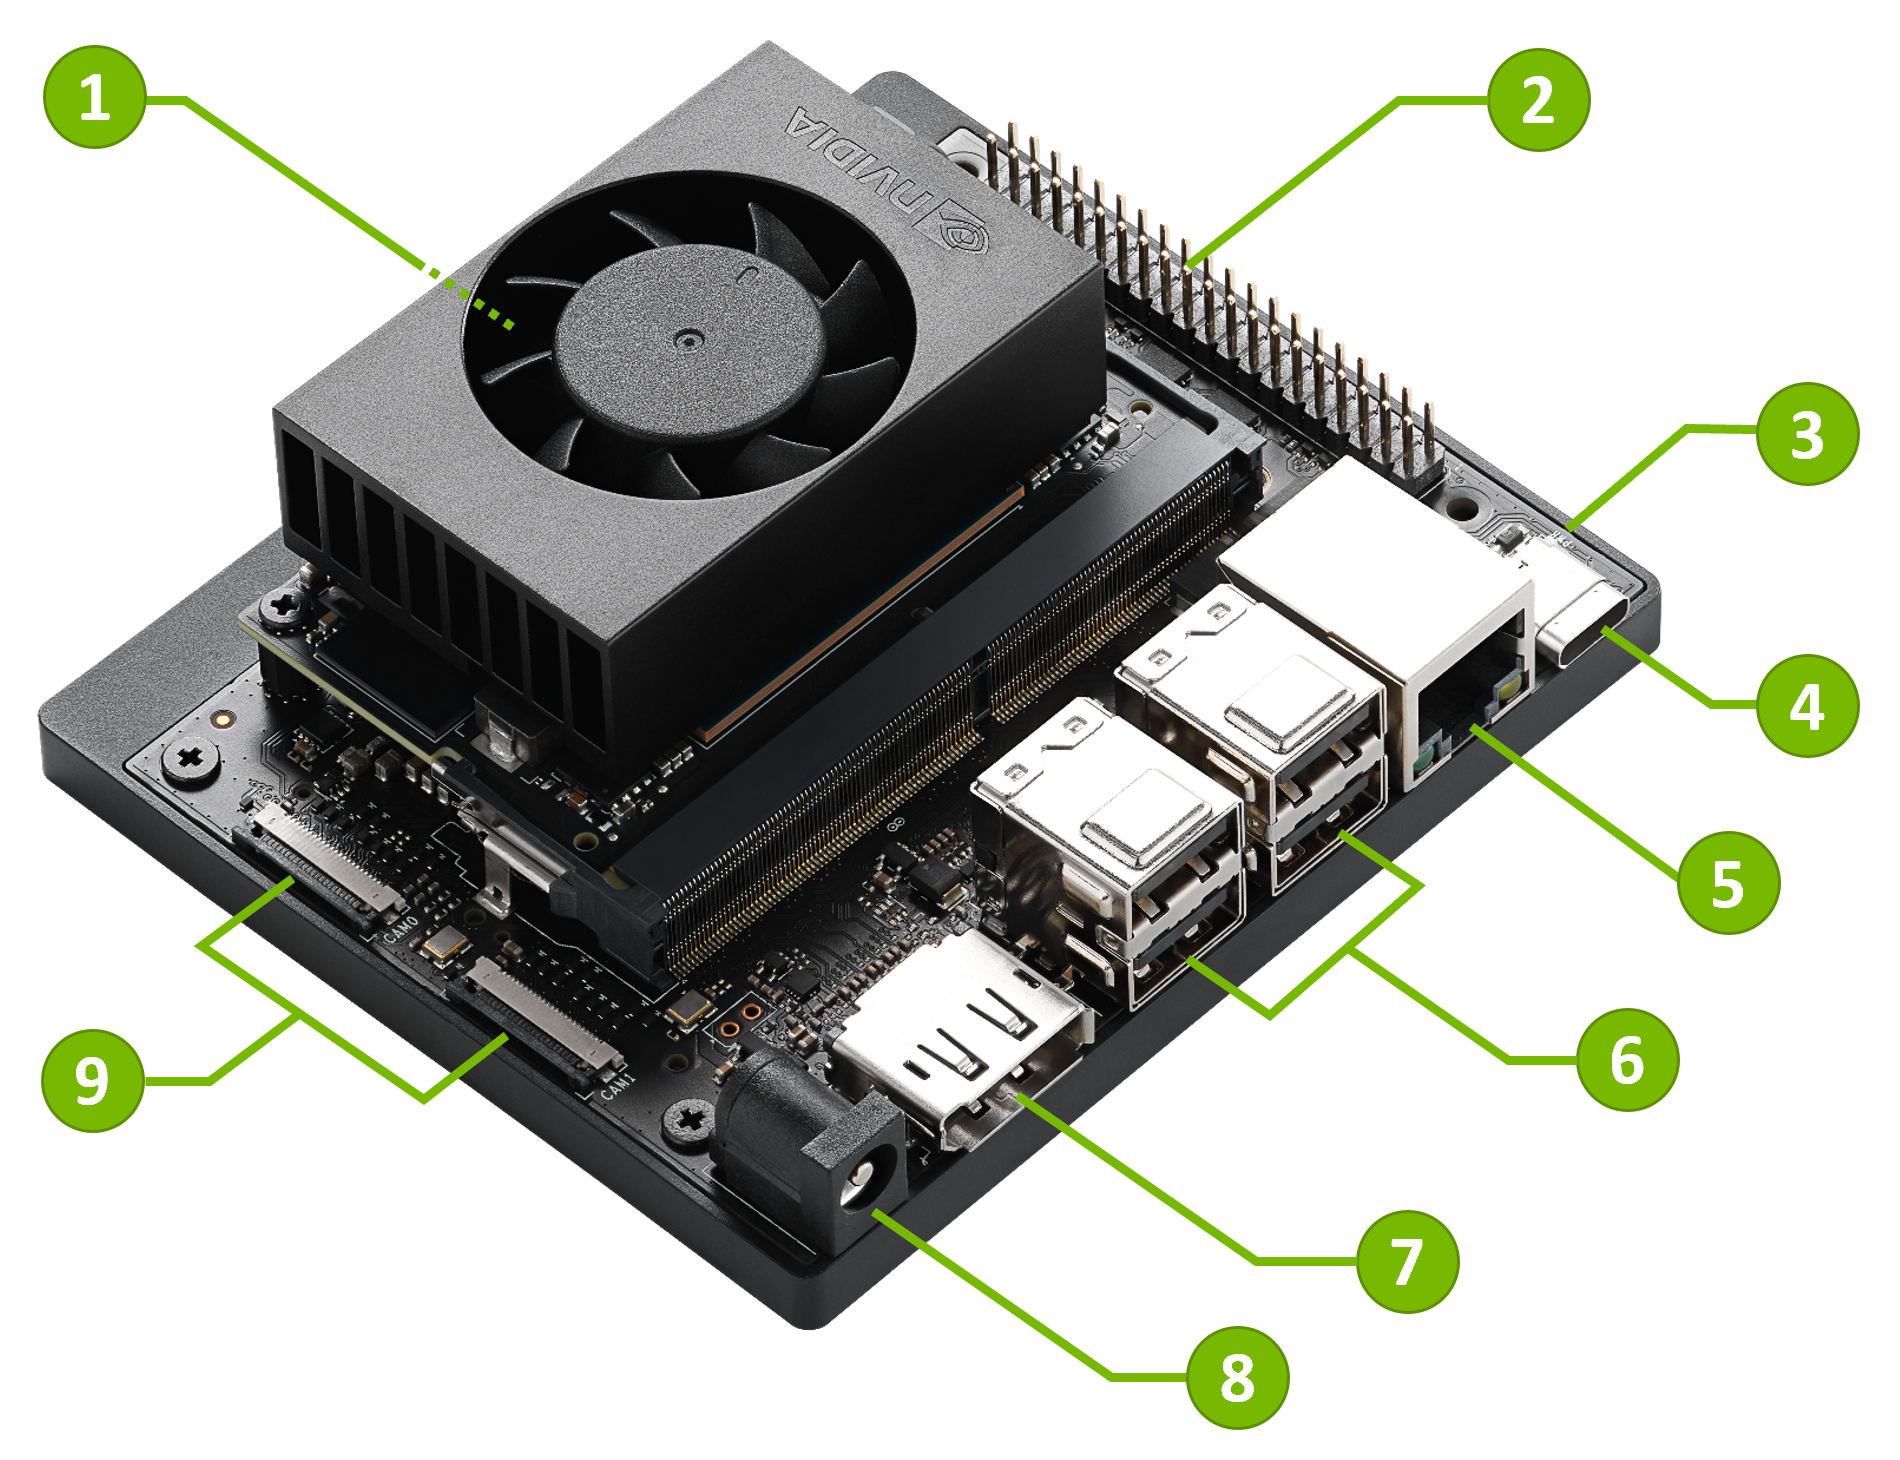
\includegraphics[width=0.8\textwidth]{Bilder/jetsonOrinNano8GB.png} 

    \caption{Jetson Orin Nano Developer Kit}
\end{figure}

\subsection*{Merkmale}

\begin{itemize}
    \item 1. microSD-Kartensteckplatz für den Hauptspeicher
    \item 2. 40-poliger Erweiterungsheader
    \item 3. Stromanzeigen-LED
    \item 4. USB-C-Port nur für Daten
    \item 5. Gigabit-Ethernet-Port
    \item 6. USB 3.1 Typ A Ports (x4)
    \item 7. DisplayPort-Anschluss
    \item 8. DC Barrel Jack für 19V Stromversorgung
    \item 9. MIPI CSI Kameraanschlüsse
\end{itemize}

\subsection*{Im Lieferumfang enthalten}

\begin{itemize}
    \item Jetson Orin Nano Modul mit microSD-Kartensteckplatz
    \item Referenzträgerplatine (inklusive 802.11 Plug-in WLAN 
    \& BT-Modul vorinstalliert mit Antenne)
    \item 19V Netzteil
    \item Eine kleine Papierkarte mit Schnellstart- und 
    Support-Informationen
\end{itemize}

\subsection*{Nicht im Lieferumfang enthalten}

\begin{itemize}
    \item microSD-Karte (empfohlen 64GB UHS-1 oder größer)
    \item USB-Tastatur und Maus
    \item Computerbildschirm
    \item USB-Kabel
    \item Zunächst ist ein Computer mit Internetverbindung und der Fähigkeit zum Flashen der microSD-Karte ebenfalls erforderlich.
\end{itemize}
\clearpage

\section{Technische Spezifikationen}
\subsection{Prozessor (CPU)}
\begin{itemize}
    \item Architektur: ARM Cortex-A78AE
    \item Kerne: 6 Kerne, bis zu 1,5 GHz
\end{itemize}

\subsection{Grafikprozessor (GPU)}
\begin{itemize}
    \item Architektur: NVIDIA Ampere, 64 Tensor Cores, 40 TOPS
\end{itemize}

\subsection{Speicher (RAM)}
\begin{itemize}
    \item 4 GB oder 8 GB LPDDR5, bis zu 68 GB/s Bandbreite
\end{itemize}

\subsection{Schnittstellen und I/O}
\begin{itemize}
    \item PCIe Gen 3 x4, USB 3.2, Gigabit-Ethernet
    \item HDMI 2.1, DP 1.2, 2x MIPI CSI-2 Kameraanschlüsse
\end{itemize}

\subsection{Leistung und Energieverbrauch}
\begin{itemize}
    \item Einstellbarer Energieverbrauch: 7 W bis 15 W
\end{itemize}

\subsection{Softwareunterstützung}
\begin{itemize}
    \item Linux for Tegra (L4T), Unterstützung für CUDA 11, C++, Python, TensorFlow, PyTorch
\end{itemize}

\section{Vergleich der Modelle}
\begin{tabular}{|l|c|c|c|}
\hline
\textbf{Modell} & \textbf{RAM} & \textbf{Leistung (TOPS)} & \textbf{Energieverbrauch} \\
\hline
Jetson Orin Nano 4GB & 4 GB & 20 TOPS & 7-15 W \\
Jetson Orin Nano 8GB & 8 GB & 40 TOPS & 7-15 W \\
\hline
\end{tabular}
\end{document}